\chapter{Appendix}
\section*{Experiment No.1}
\subsection*{Germanium}
\begin{figure}[h]
\begin{center}
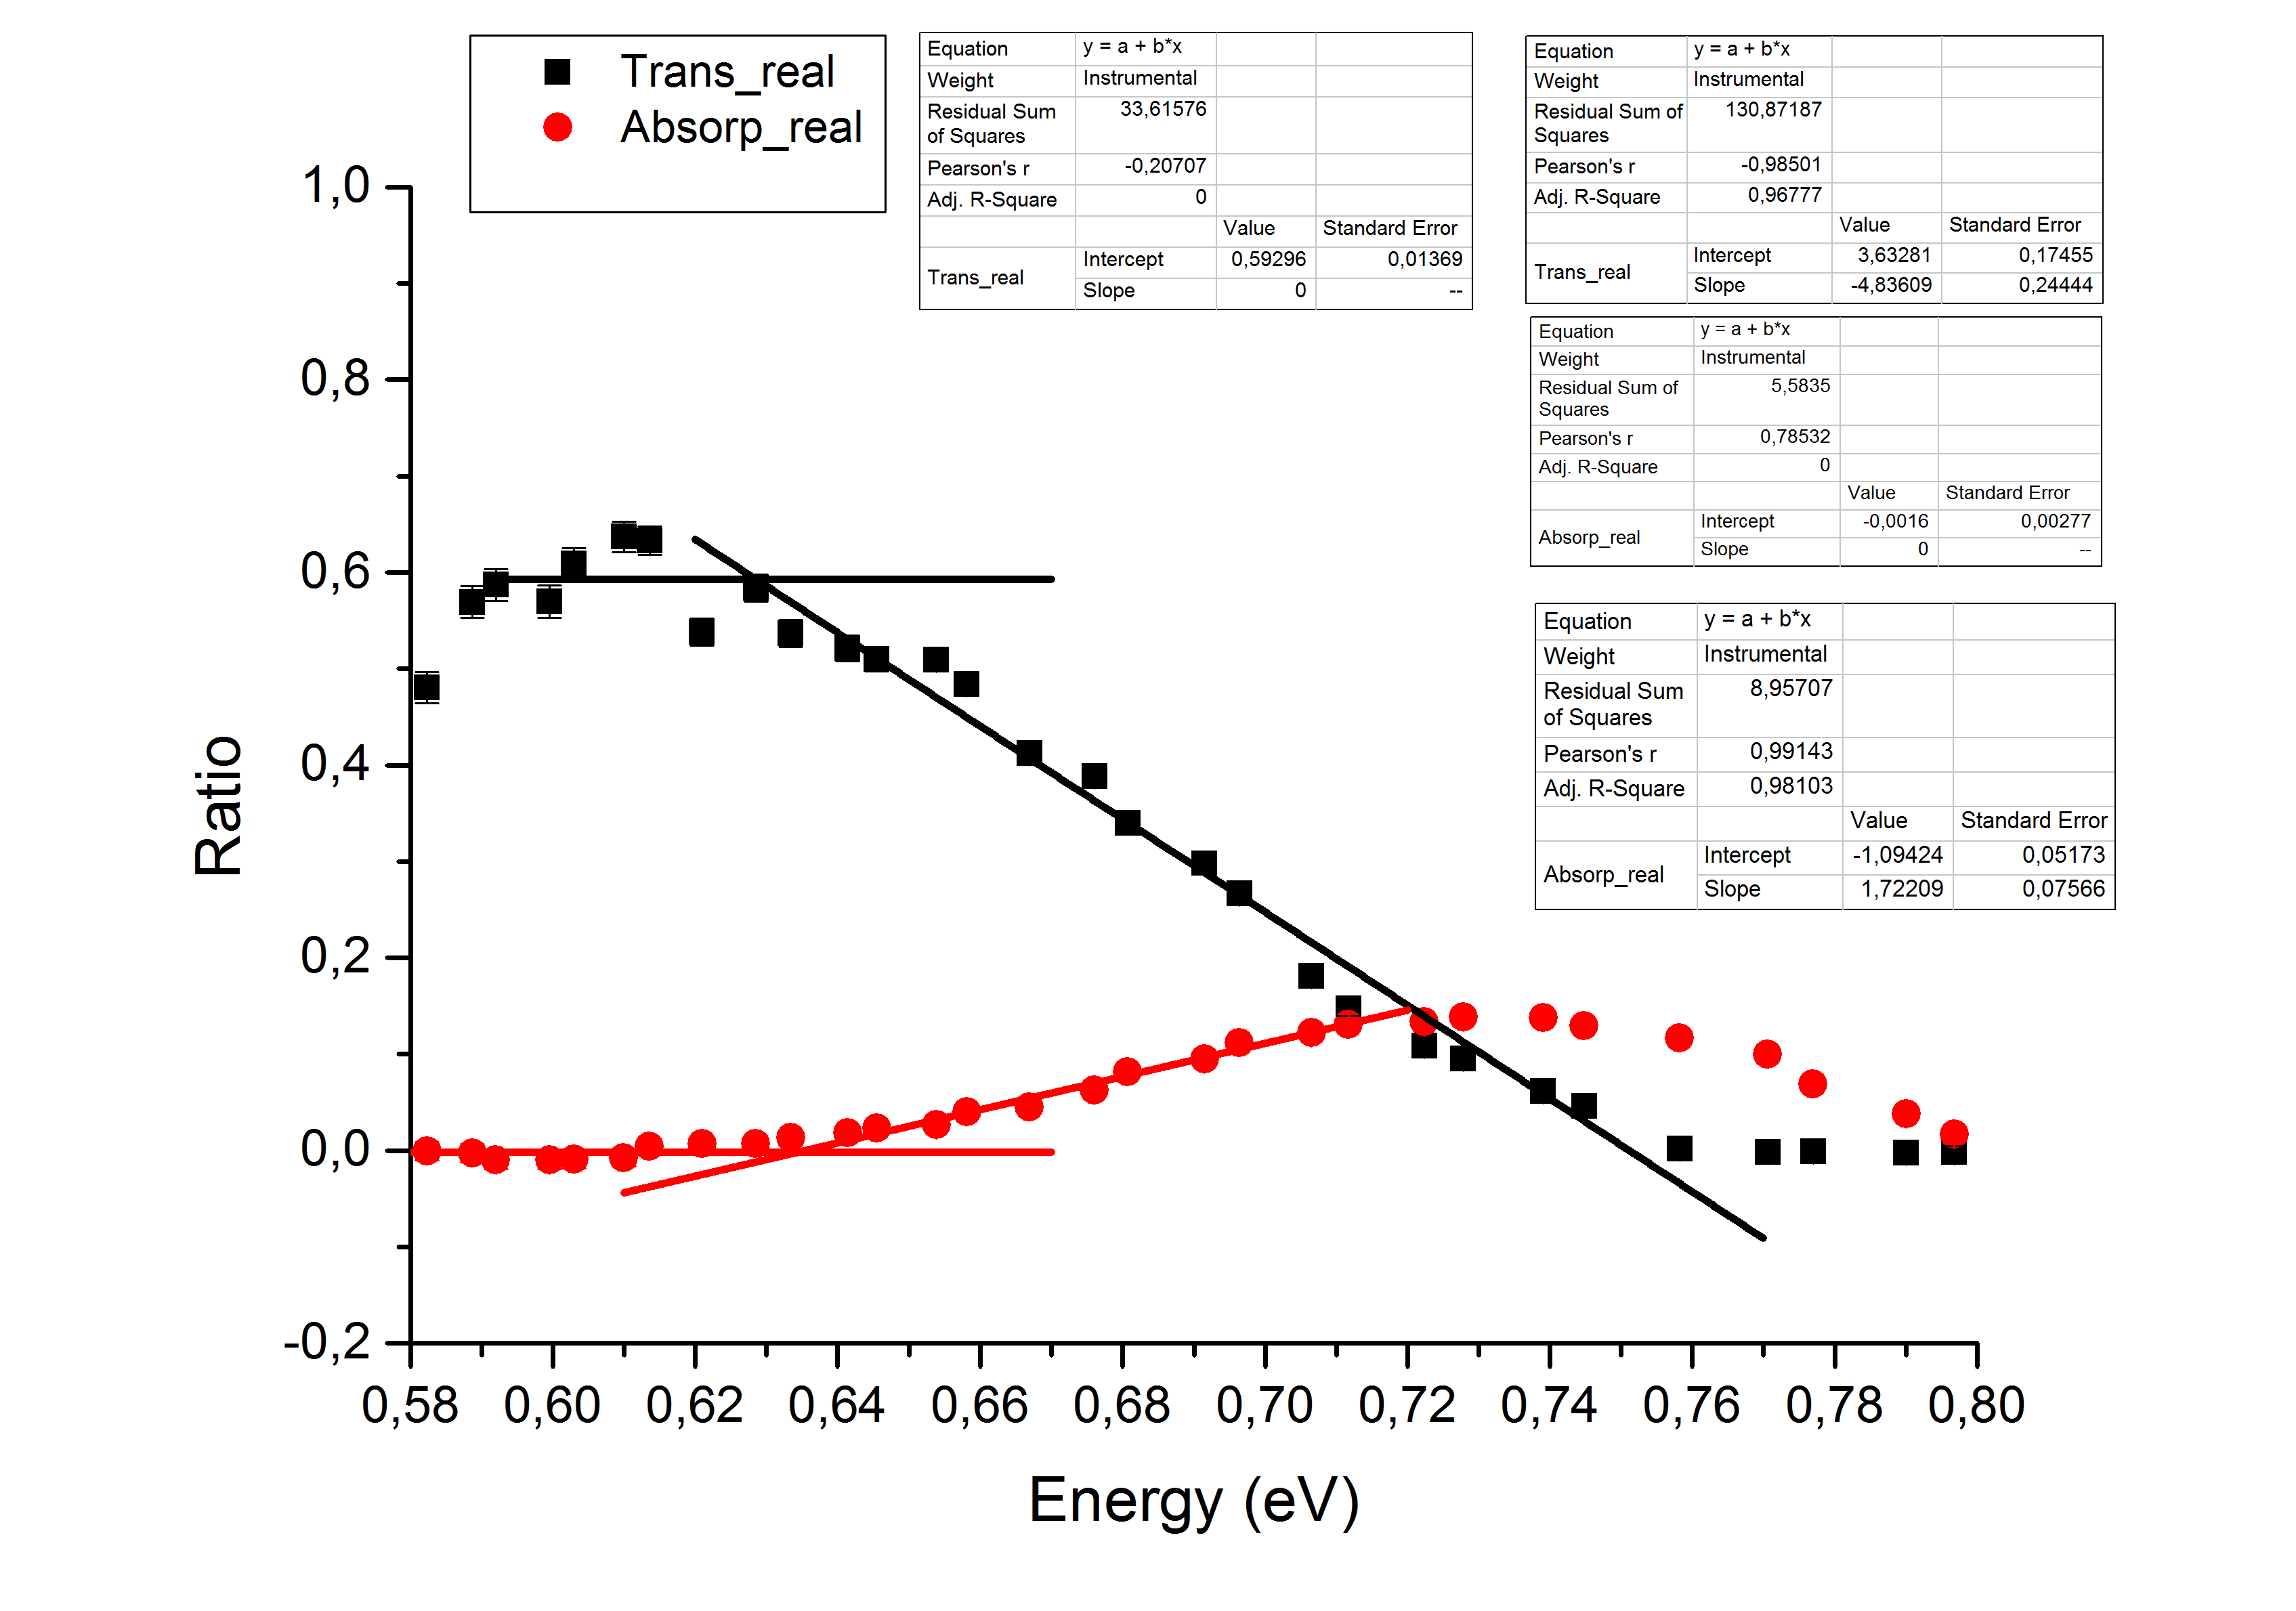
\includegraphics[scale=0.25]{Bilder/Teil1/V1_Ge_positiv}
\caption{Positive fit section of Germanium}
\label{fig:GePo}
\end{center}
\end{figure}
\begin{figure}[h]
\begin{center}
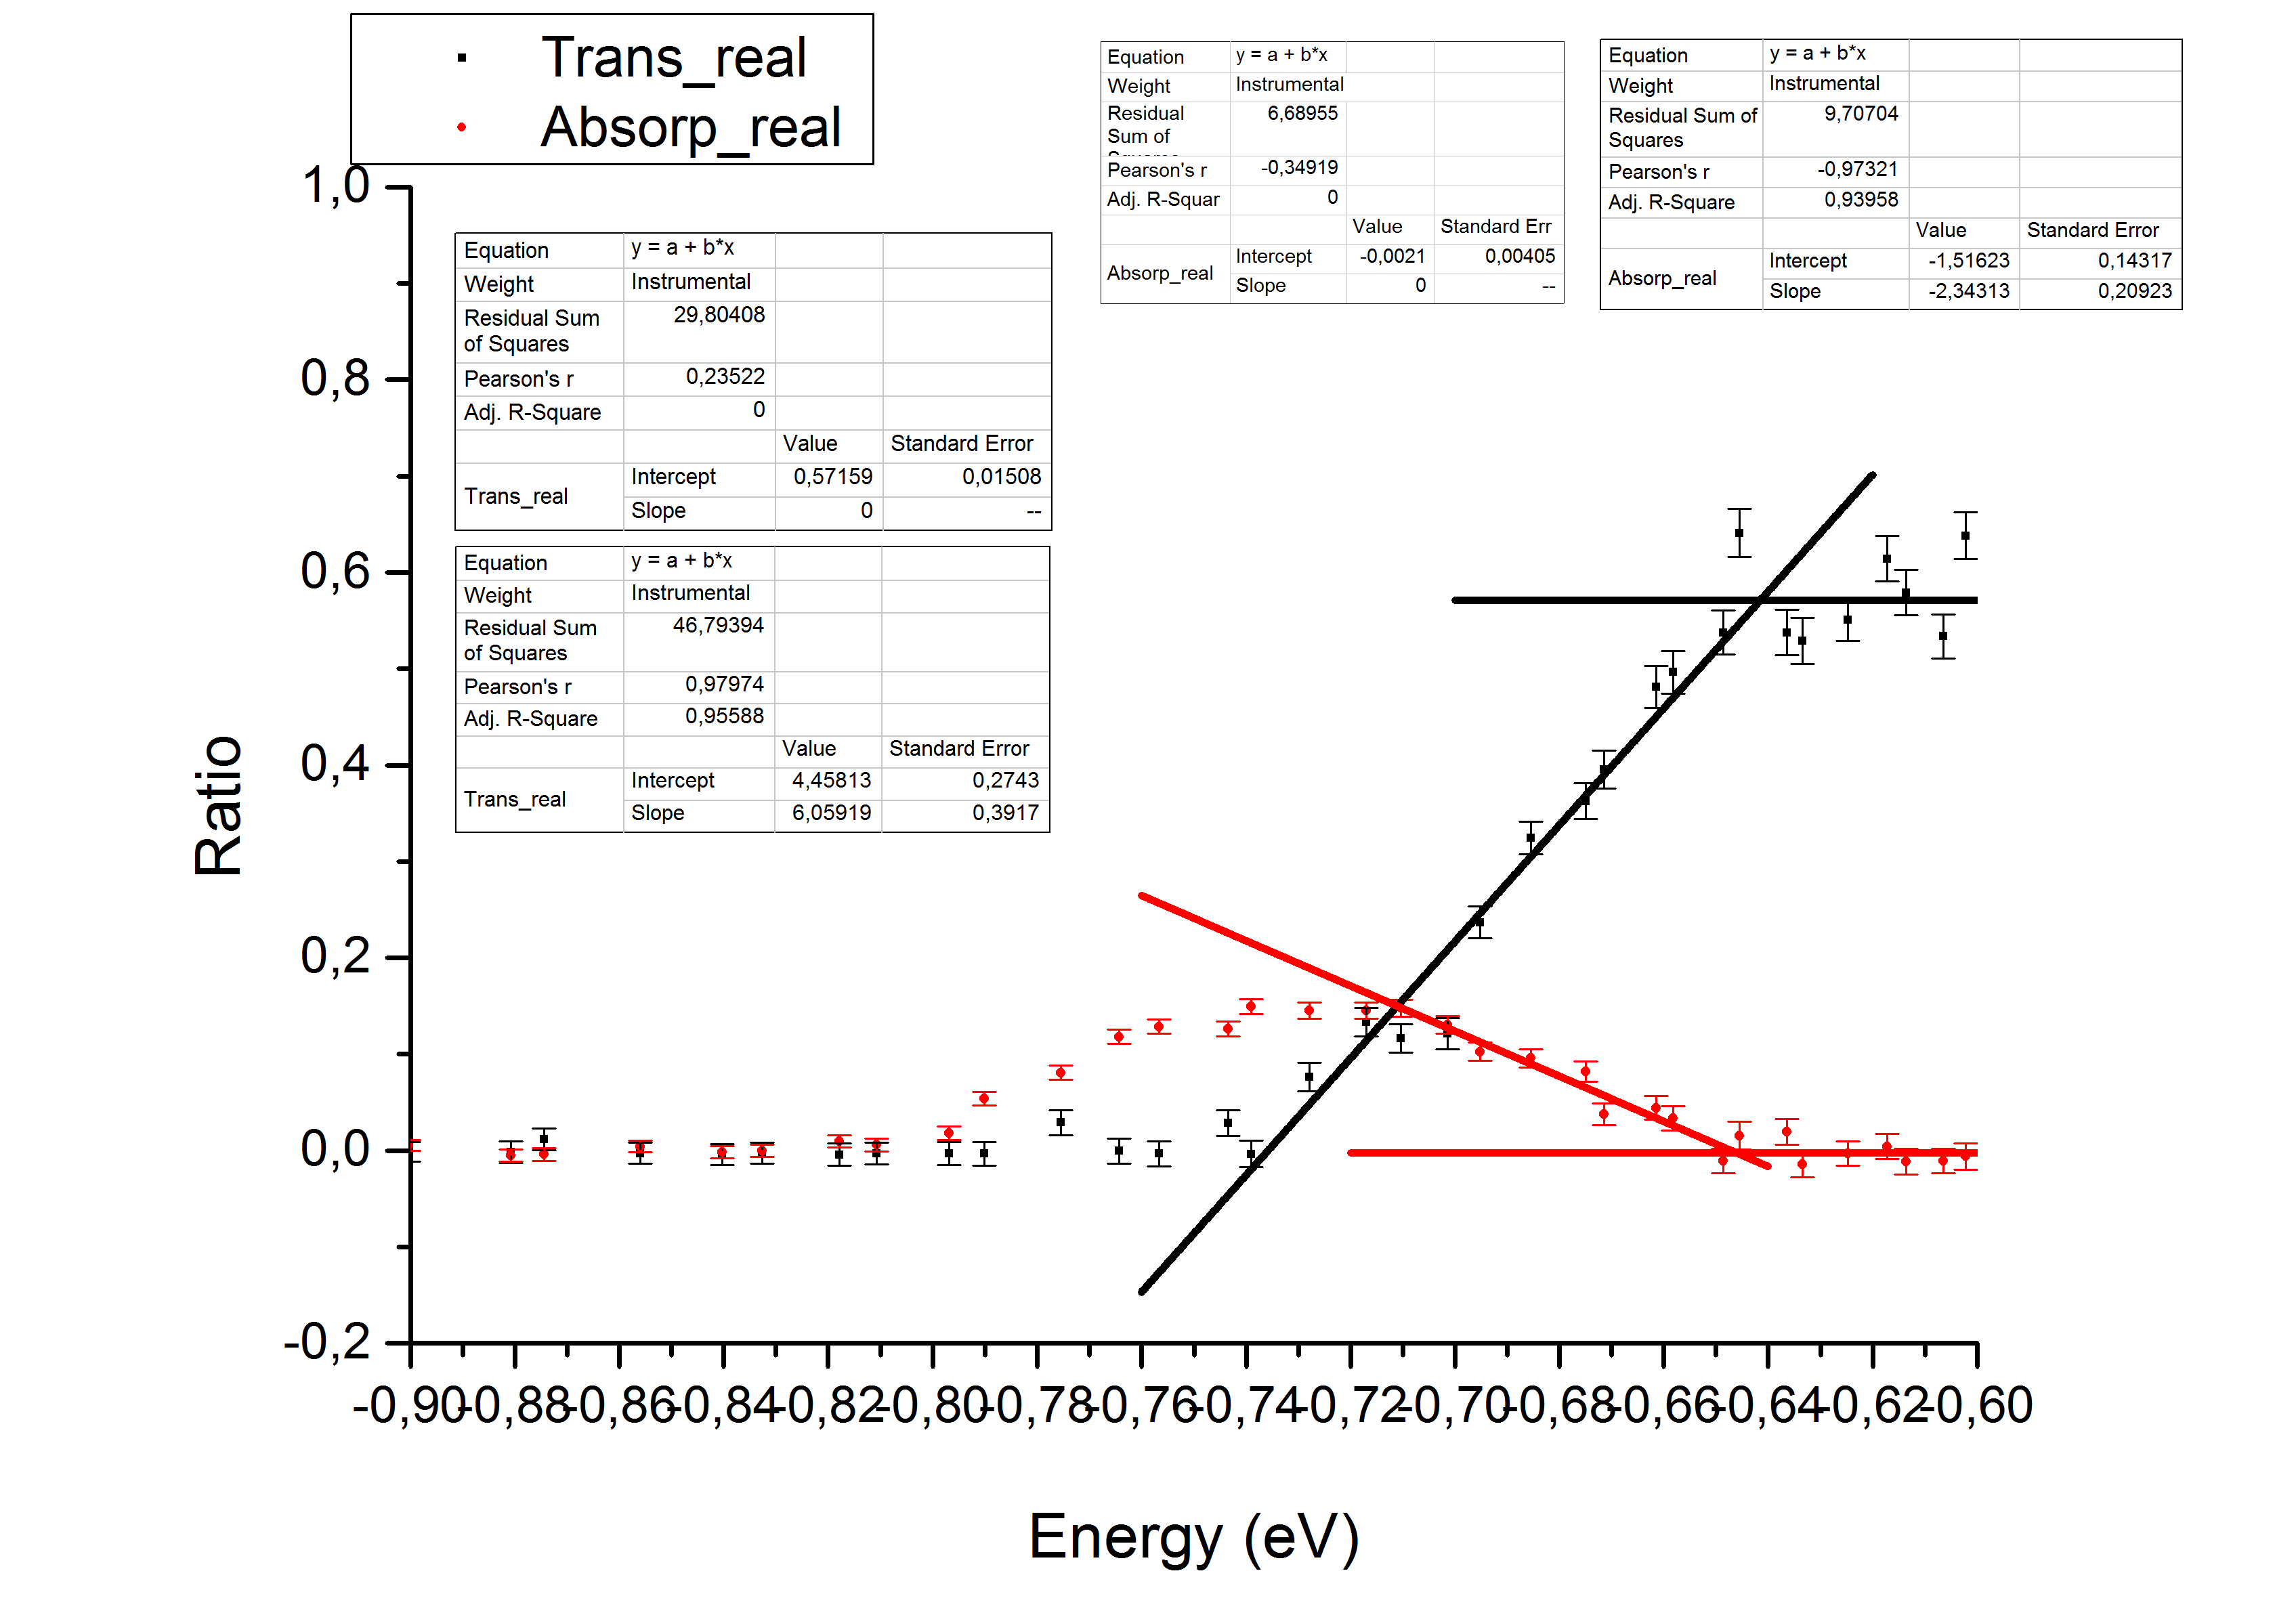
\includegraphics[scale=0.25]{Bilder/Teil1/V1_Ge_negativ}
\caption{Negative fit section of Germanium}
\label{fig:GePo}
\end{center}
\end{figure}
\subsection*{Silicon}
\begin{figure}[h]
\begin{center}
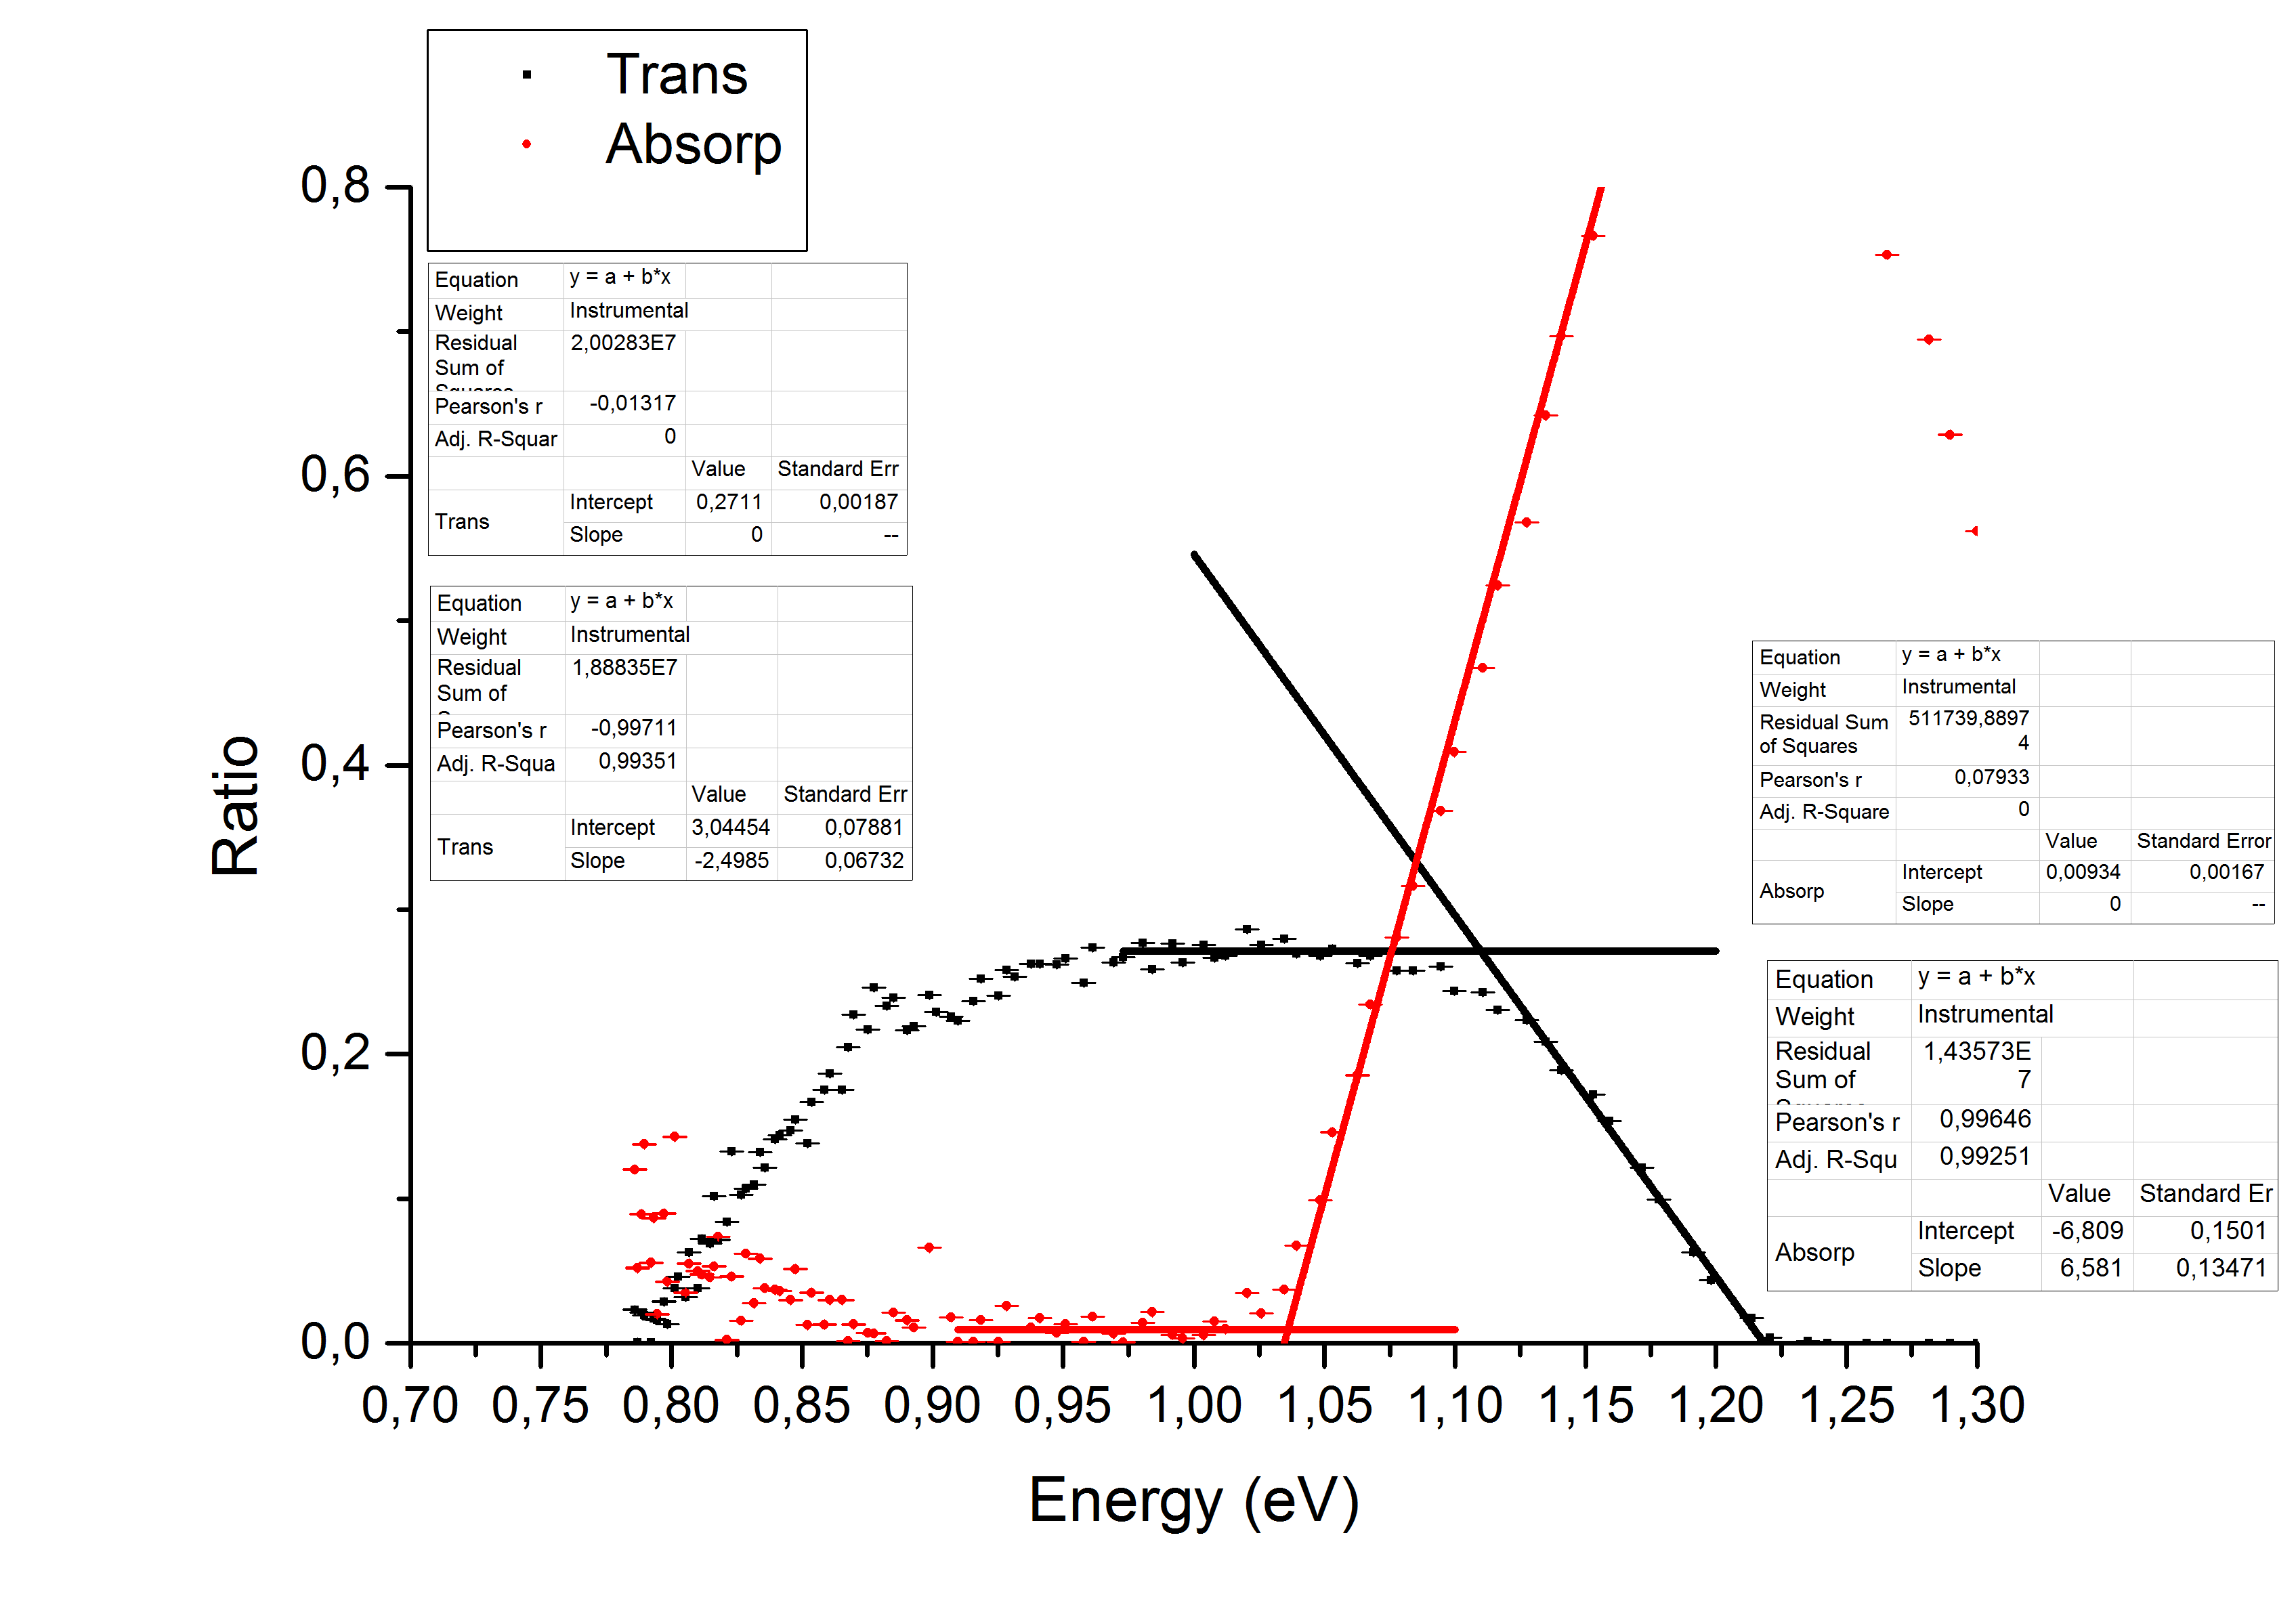
\includegraphics[scale=0.25]{Bilder/Teil1/V1_Si_positiv}
\caption{Positive fit section of Silicon}
\label{fig:SiPo}
\end{center}
\end{figure}
\begin{figure}[ht!]
\begin{center}
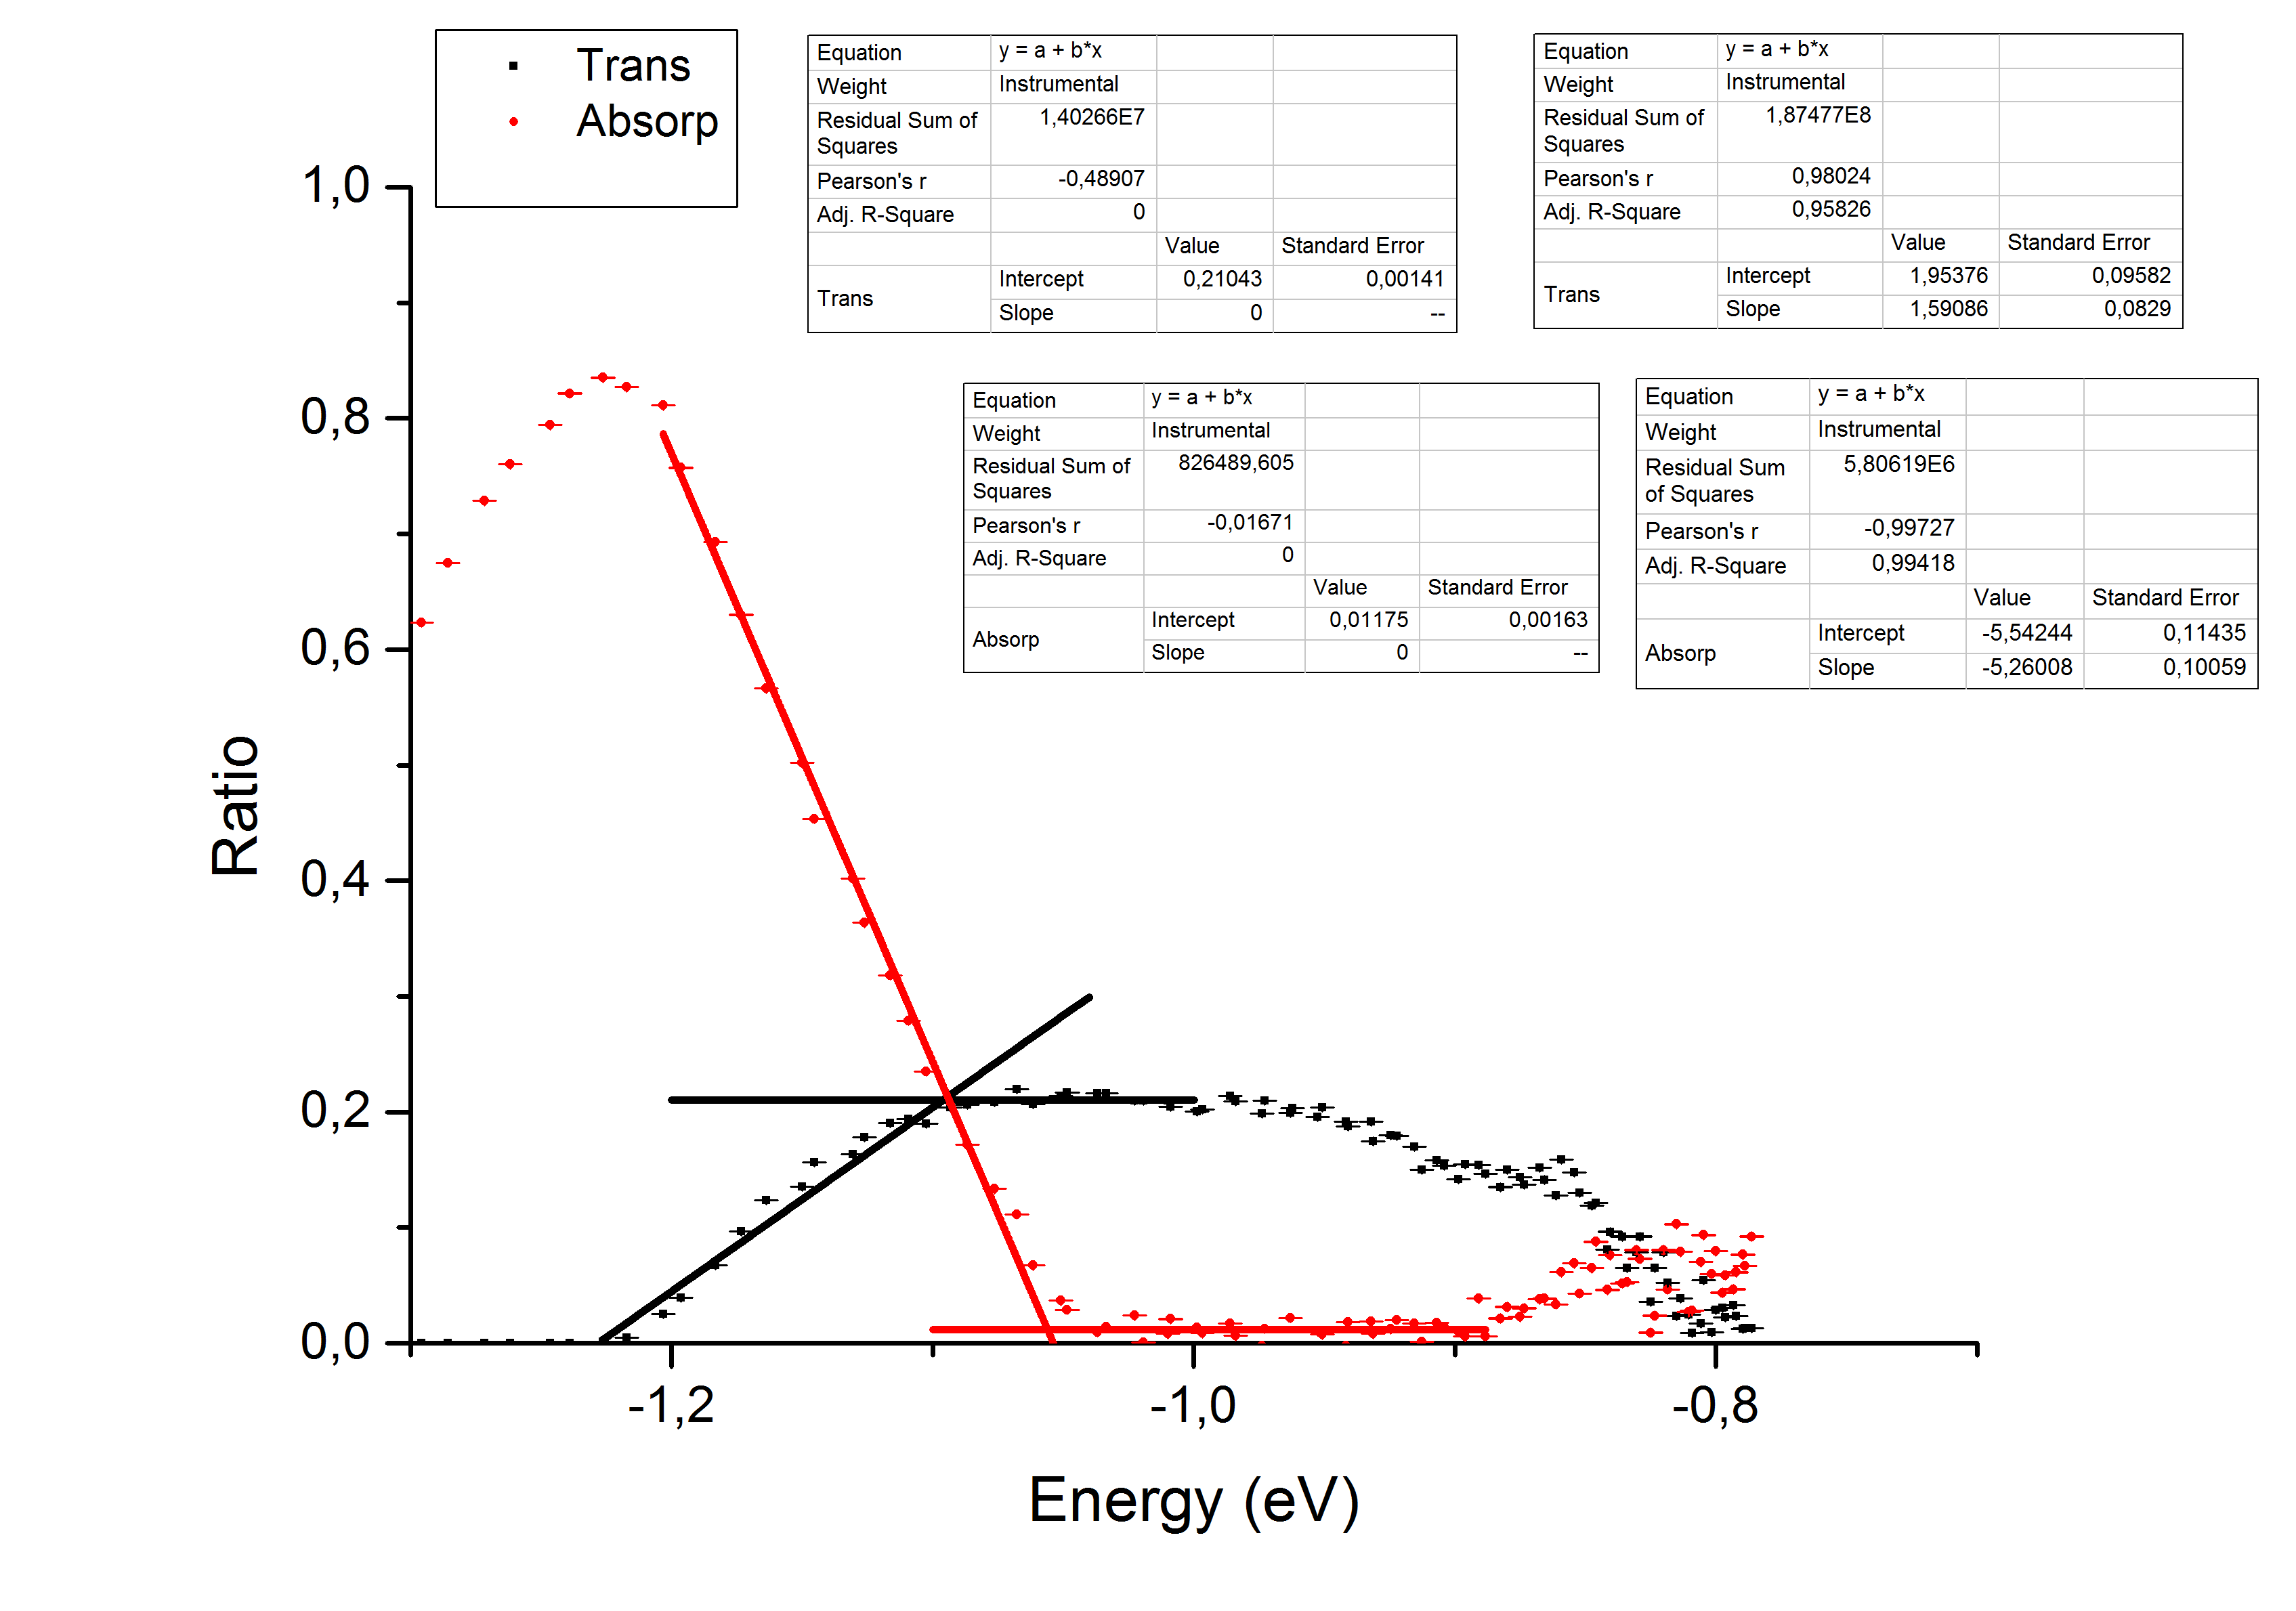
\includegraphics[scale=0.25]{Bilder/Teil1/V1_Si_negativ}
\caption{Negative fit section of Silicon}
\label{fig:SiNe}
\end{center}
\end{figure}